\chapter{Gestión de la Base de datos del HUVR} \label{cap:02Datos}

La base de datos empleada en el Trabajo Fin de Grado es una combinación del Registro S31 y S32 del Hospital Universitario Virgen del Rocío, que contiene información sobre consultas realizadas a pacientes de cáncer de pulmón. La base de datos fue adaptada por el equipo técnico y montada en una pequeña base de datos PostgreSQL para permitir su uso en el proyecto. 

La tarea de OMOPizar la base de datos ha sido realizada por mi compañero Francisco Rey Garduño como objeto de su Trabajo de Fin de Grado ''Análisis de datos sanitarios mediante herramientas OHDSI y modelo de datos OMOP''.


\section{Estructura de la BD del HUVR}

La base de datos se ha implementado con una estructura PostgreSQL. Para acceder a ella se ha utilizado el administrador de bases de datos pgAdmin 4.0. 

Dentro del servidor HUVR al que se proporcionó acceso, la base de datos corresponde a \code{omop\_oncologia}, tal y como se muestra en la Figura \ref{figure:servidorHUVR}. Esta base de datos presenta seis esquemas de los cuales \code{omop}, \code{result} y \code{temp} son relevantes para el análisis y se describen a continuación:

\begin{itemize}
    \item \textbf{\code{omop}}. Este esquema almacena todas las tablas con la toda la información omopizada de los pacientes y eventos clínicos de la base de datos.
    \item \textbf{\code{result}}. Este esquema almacena los resultados de ejecutar ACHILLES (véase \ref{sec:07herramientas} ''Herramientas de OHDSI'') sobre la base de datos. Es crucial para la correcta integración de la base de datos con ATLAS.
    \item \textbf{\code{temp}}. Este esquema almacena información temporal durante las ejecuciones de ACHILLES.
\end{itemize}

La base de datos contiene 1332 instancias de pacientes registradas, como se muestra en la Figura ''Captura de pantalla de pgAdmin del número de instancias de la tabla \code{person}''.

\begin{figure}[H]
    \centering
    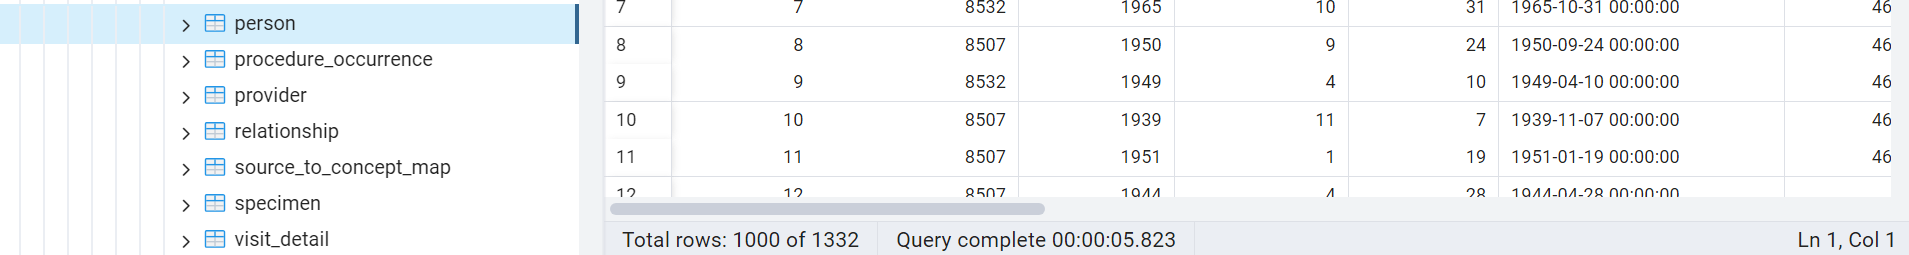
\includegraphics[width=0.90\textwidth]{figures/personCount.png}
    \caption{Captura de pantalla de pgAdmin del número de instancias de la tabla \code{person}}
    \label{figure:personCount}
\end{figure}

\begin{figure}[H]
    \centering
    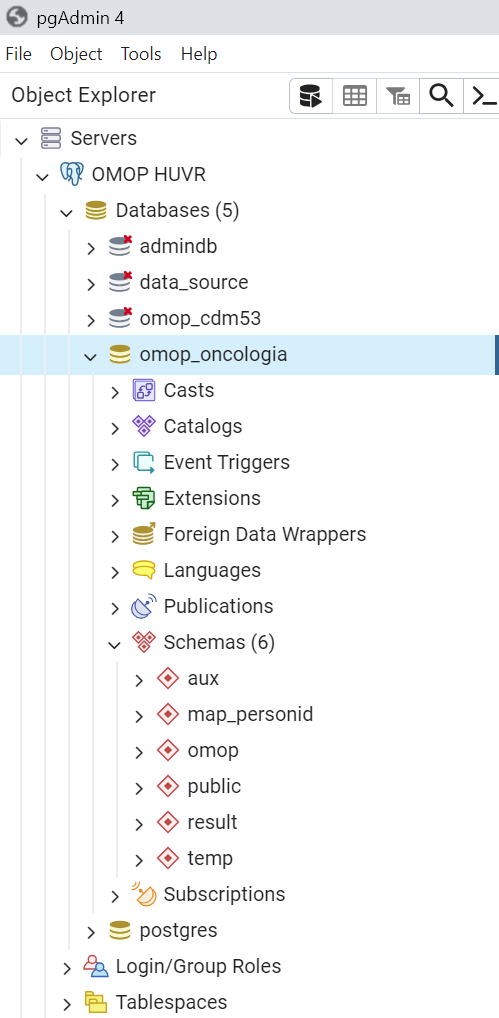
\includegraphics[width=0.50\textwidth]{figures/servidorHUVR.png}
    \caption{Captura de pantalla de pgAdmin de la estructura del servidor del HUVR}
    \label{figure:servidorHUVR}
\end{figure}


\section{Integración de la BD en ATLAS Broadsea}

El proceso de integración de una base de datos externa en la WebAPI de Broadsea se describe con gran detalle en el Anexo \ref{anexo:manual} ''Manual de instalación, despliegue y configuración de ATLAS Broadsea''. No obstante, en esta subsección se presenta de forma sencilla el proceso de conexión con la base de datos del HUVR.

Para establecer la conexión con una base de datos externa se debe registrar la base de datos en el esquema de la WebAPI de Broadsea, concretamente en las tablas \code{source} y \code{source\_daimon}. Para ello se ejecuta un conjunto de queries disponibles en el archivo del repositorio de github \code{Thesis-ATLAS-OHDSI/files/thesis/sql/queries\_insert\_huvr\_source.sql}. 

En las Figuras \ref{figure:sourceHUVR} ''Captura de pantalla de pgAdmin de la tabla \code{source}'' y \ref{figure:source_daimonHUVR} ''Captura de pantalla de pgAdmin de la tabla \code{source\_daimon}'' se muestran los resultados de la ejecución correcta de las queries. 

\begin{figure}[H]
    \centering
    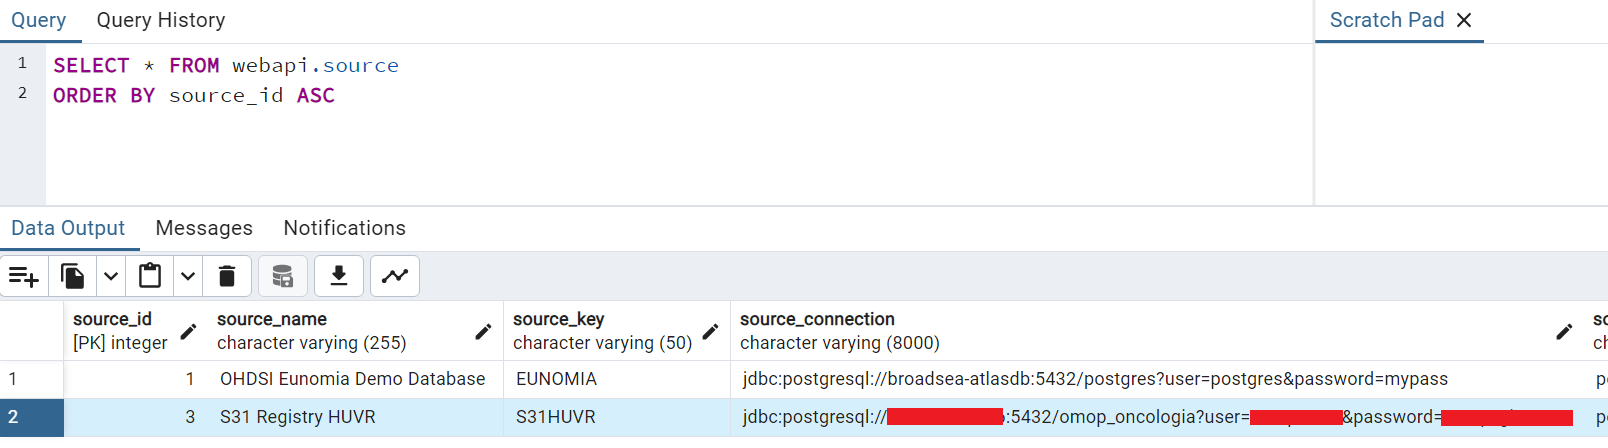
\includegraphics[width=0.90\textwidth]{figures/sourceHUVR.png}
    \caption{Captura de pantalla de pgAdmin de la tabla \code{source}}
    \label{figure:sourceHUVR}
\end{figure}

\begin{figure}[H]
    \centering
    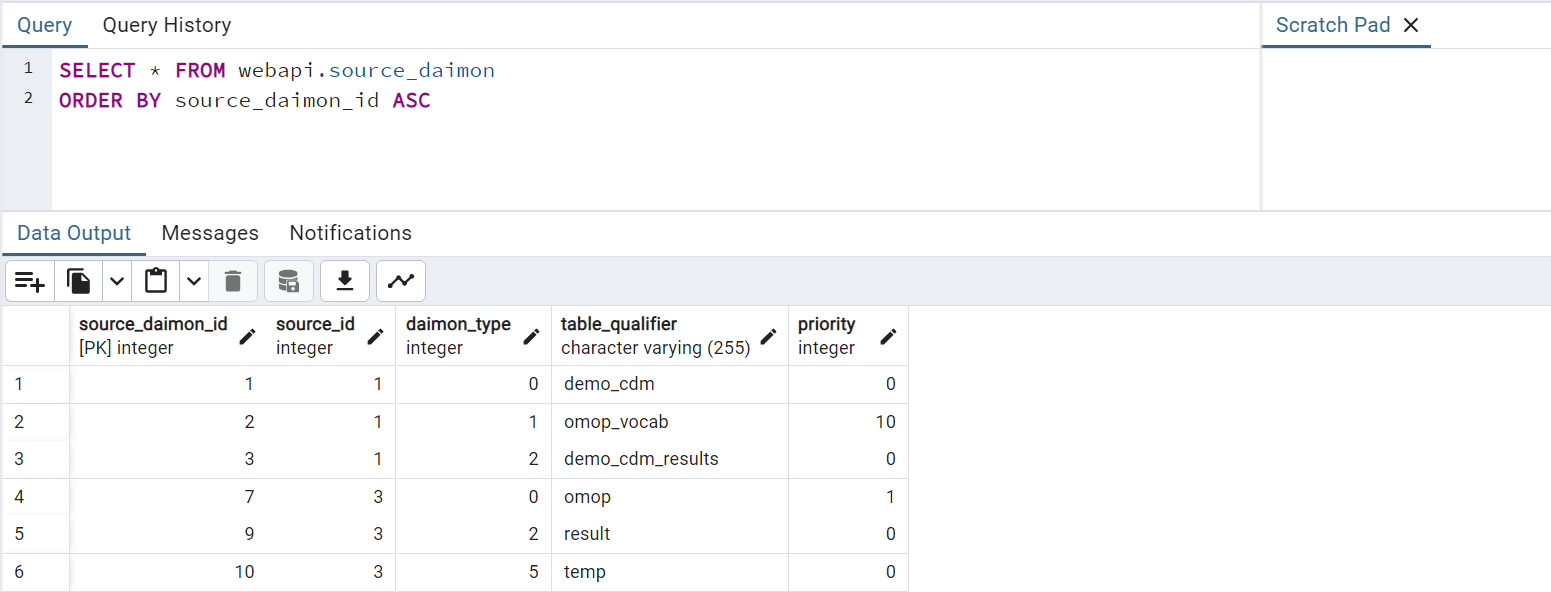
\includegraphics[width=0.75\textwidth]{figures/source_daimonHUVR.png}
    \caption{Captura de pantalla de pgAdmin de la tabla \code{source\_daimon}}
    \label{figure:source_daimonHUVR}
\end{figure}

Se puede comprobar que la integración de la base de datos en Broadsea se ha realizado correctamente a través del menú \code{configuration} de ATLAS, donde se muestran los detalles de las bases de datos integradas con la herramienta. En la Figura \ref{figure:configATLAS} ''Captura de pantalla de menú \code{configuration} de ATLAS Broadsea'' se observa que hay dos bases de datos: la base de datos de Eunomia que viene preinstalada con Broadsea y la base de datos recién instalada.

\begin{figure}[H]
    \centering
    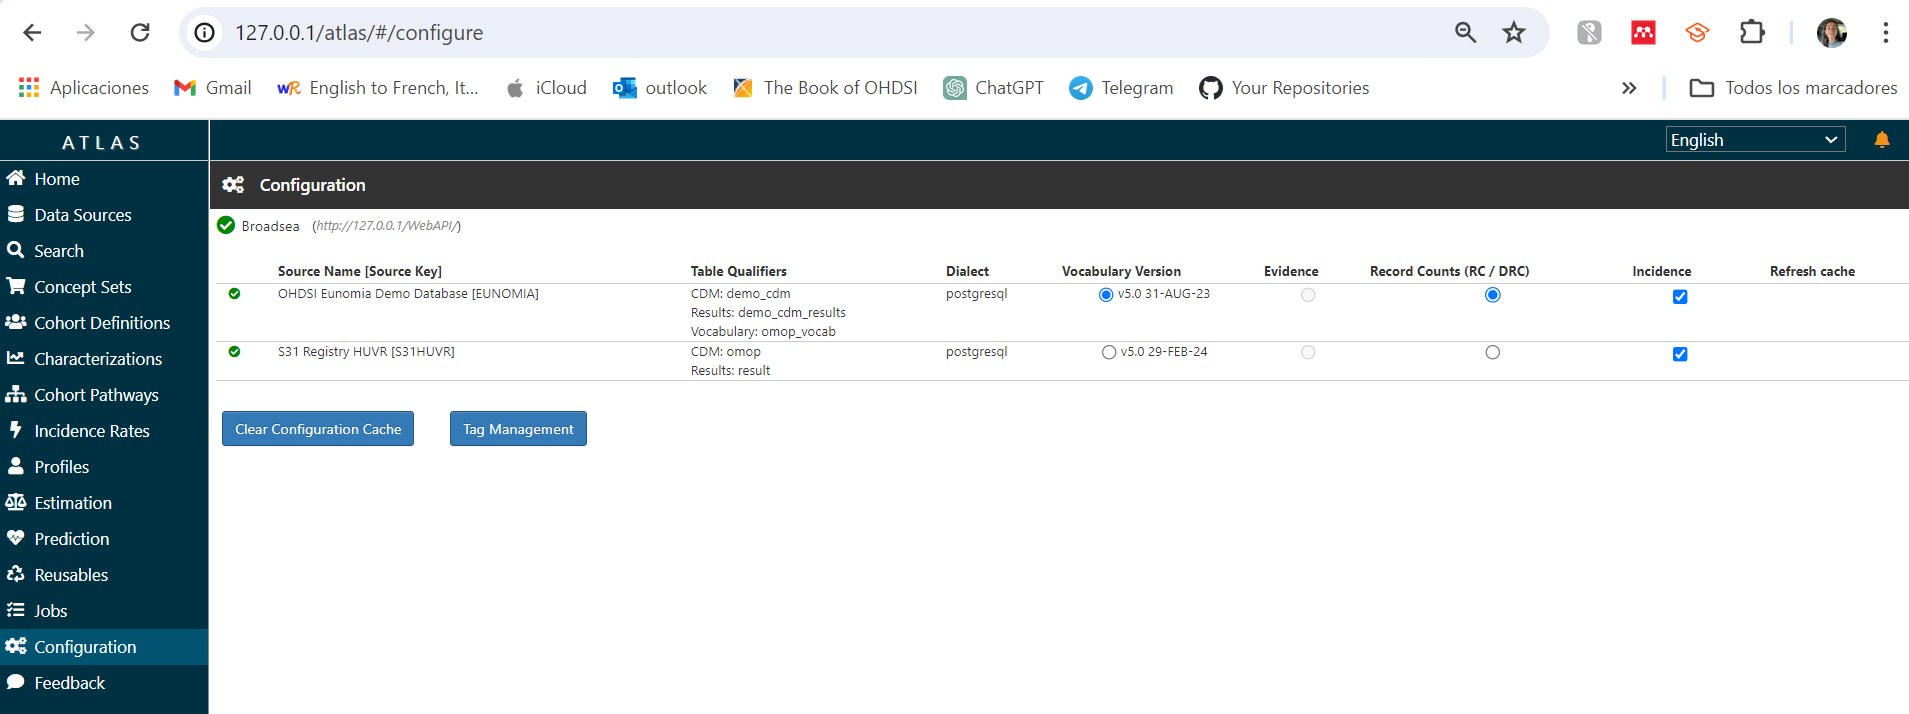
\includegraphics[width=0.90\textwidth]{figures/configATLAS.png}
    \caption{Captura de pantalla de menú \code{configuration} de ATLAS Broadsea}
    \label{figure:configATLAS}
\end{figure}